\chapter{What you don't see can hurt you: how imperceptible signals shape what we see}
\ifpdf
    \graphicspath{{chapter3/chapter3-figs/PNG/}{chapter3/chapter3-figs/PDF/}{chapter3/chapter3-figs/}}
\else
    \graphicspath{{chapter3/chapter3-figs/EPS/}{chapter3/chapter3-figs/}}
\fi

\renewcommand{\runningTitle}{Stereopsis: what you don't see can hurt you}
\markboth{\MakeUppercase{\thechapter. \runningTitle }}{\thechapter. \runningTitle}

% TODO
% replace citations [done] [needs checking]
% replace figure references [done] [needs checking]

\section{Introduction}

Sir Charles Wheatstone \cite{Wheatstone:1838xf} aquatinted the world with the glories of binocular vision. Through practical demonstration of the stereoscope, he broadcast his insight that differences between the two eyes' retinal images provide precise information about three-dimensional (3D) shape. Modern treatments of stereopsis, in both artificial- and biological- systems, have emphasised the need to identify similarities between the eyes to understand 3D vision. This is captured as the ``binocular correspondence problem'' \cite{JULESZ:1964ff,Marr:1976dq,Scharstein:2002by} that entails matching the same image features between the two eyes so that the difference in retinal positions can be extracted. 

The potential difficulties of binocular matching were made stark by random dot stereogram (RDS) displays \cite{JULESZ:1964ff}. Here, observers perceive a coherent 3D shape, despite viewing monocular images that contain no meaningful structure. Given that the elements making up the display are self-similar, there is huge potential for the brain to match up the ``wrong'' parts of the display. Yet, viewers typically perceive compelling 3D forms without much difficulty. The logical interpretation of these stimuli was, therefore, that the brain is faced with a hard problem in identifying the one ``correct match'' in a sea of ``false matches'' that conflate signals originating from locations in 3D space.

This intuition has guided thinking to ask how the brain could find the correct match. However, as I have alluded to in Chapter 2, the more pertinent question is to consider the best way for neurons to extract statistical information about the depth structure of the scene \cite{Goncalves:2017aa}. In particular, potentially valuable information is conveyed by neural signals that appear discordant with perceptual experience. Moreover, the properties of binocular neurons are not particularly well-suited to identifying ``correct'' matches per se: many respond best to different features in the two eyes \cite{DeAngelis:1991mb,Prince:2002uq,Tsao:2003pi}. This includes tuning to ``anticorrelated'' stimuli (Fig. \ref{fig:c2f1}a) that are contrast-inverted between the eyes (i.e., a bright feature in one eye's image corresponds to a dark feature in the other) \cite{Ohzawa:1990cq,Cumming:1997ve}.

On the basis that the brain seeks to identify ``correct'' matches, it is very puzzling that the brain responds to anticorrelated stimuli: in general, a single physical feature in the environment will not project opposite contrast images into the two eyes. Moreover, viewing anticorrelated stimuli leads to a discombobulating perceptual experience such that it has long been thought that observers are essentially blind to the information depicted in anticorrelated RDS \cite{BLTJ:BLTJ3954,Cogan:1993yr,Cumming:1998ib,Read:2000kx,Hibbard2014}.

Here I demonstrate that the traditional focus on ``correct'' matches fails to capture the signals used by human visual system. In particular, I show that anticorrelated signals --- traditionally viewed as ``false'' --- are, in fact, perceptually informative. I do this by mixing correlated and anticorrelated elements together to reveal profound consequences for perception. Specifically, I provide evidence that the disparity information carried by anticorrelated features (itself imperceptible) masks correlated features. This masking effect is contingent upon (i) the disparity of the anticorrelated features, (ii) the magnitude of the disparity, (iii) the spatial configuration of binocular correlation, and (iv) the relative onset timing of anticorrelated and correlated elements.

This demonstrates the utility of signals that we know are carried by V1 neurons, but which, to this point, have been regarded as a nuisance signal that should be filtered out. I show that the brain is sensitive to information that one ``cannot see'' and it uses these signals to shape perceptual judgments. This is compatible with the idea that neural sensors for mismatched features provide a principled means of acquiring more information about the depth structure of the viewed scene \cite{Goncalves:2017aa}, as predicted by the end of Chapter 2. These mismatches provide proscriptive ``what not'' information to drive suppression of unlikely interpretations of the viewed scene.


\section{Methods}
\subsection{Participants}
Participants had normal or corrected-to-normal vision, were screened for stereo deficits, and provided written informed consent. All procedures were approved by the University of Cambridge ethics committee. For Experiment 1, I tested 12 participants (4 females; aged between 21 and 41 years). Three participants (including the two authors) were tested in experiments 2-4.

\subsection{Main experiment}
In Experiment 1, I presented stereoscopic stimuli using a stereoscope equipped with two Samsung 2233 LCD displays (1680 x 1080 pixels, refreshed at 120 Hz) driven by an NVIDIA Quadro 4000 graphics card. The monitors were placed laterally and were viewed using a pair of infrared permeable mirrors. The viewing distance was 50 cm, yielding a resolution of 31 pixels per degree of visual angle. The position of each eye was recorded using an EyeLink 2000 video eye tracker at a sampling rate of 1000 Hz.

I used MATLAB (The Mathworks Inc., Natick, USA) and Psychtoolbox \cite{Brainard:1997aa,Pelli:1997aa,kleiner2007s} for generating and delivering stimuli. Stimuli were random-dot stereograms (RDS) composed of black and white dots on a mid gray background. The RDS (\ang{7}x\ang{7}) was presented within a circular aperture (\ang{11} radius) surrounded by a pink noise pattern. Each dot subtended approximately 4 minutes of arc and the dot density was 96 dots/deg\textsuperscript{2}. No occlusion between the dots was permitted. Stimuli were presented for 300 milliseconds. The displays were luminance calibrated and the display outputs linearised.

The dots in the RDS could be either correlated or anticorrelated between the eyes. Binocular disparity was defined according to a step edge configuration, where the left and right halves of the stereograms had opposite disparity sign (Fig. \ref{fig:c2f1}a;  3 arcmin). I rendered stimuli such that (i) correlated and anticorrelated dots had the same disparity configuration (Fig. \ref{fig:c2f1}a, ``same'' condition) or (ii) correlated and anticorrelated dots had the opposite disparity configuration (Fig. \ref{fig:c2f1}a, ``opposite'' condition). Observers were asked to report which half of the stereogram they perceived closest in depth. I varied the proportion of correlated to anticorrelated dots according to a QUEST procedure \cite{Watson:1983aa} set to estimate 75\% correct thresholds for the ``same'' and ``opposite'' disparity sign conditions (2 runs; 100 trials per run).
To control for the possibility that anticorrelated dots carried a perceivable depth signal per se, I collected 200 additional trials where the QUEST stimuli were ``replayed'' exclusively with the correlated dots or the anticorrelated dots. I then quantified the proportion of correct responses for correlated and anticorrelated stimuli. 

\subsection{Subsequent experiments}
Experiments 2-4 sought to characterize the masking effect with high spatial and temporal precision. To this end, I used a modified Wheatstone stereoscope with a long viewing distance (170 cm) and high temporal resolution display (ViewPixx 3D monitor, VPixx Technologies Inc., Saint-Bruno, Canada) driven by a NVIDIA Quadro FX 5600 (1920 x 1080 pixels; refresh rate = 120 Hz). The left and right images were presented side-by-side on a single screen, ensuring that the binocular images were synchronized. The display resolution was 110 pixels per degree.

RDS stimuli (\ang{5}x\ang{5}) were presented within a central aperture (\ang{8}) surrounded by a random pink noise pattern. Each stereogram contained a mixture of black and white dots on a mid gray background. Each dot subtended approximately 4 arcmin and the dot density was 85 dots/deg\textsuperscript{2}. No occlusion between the dots was permitted. On each trial, stimuli were presented for 300 milliseconds. The display was luminance calibrated and the display outputs linearised.

\subsection{Experiment 2: The effect of disparity offset between correlation and anticorrelation in depth}
In Experiment 1, I contrasted performance when correlation and anticorrelation carried the same or opposite disparity signs. In Experiment 2, I parametrically varied the difference between the disparities of correlated and anticorrelated dots. The correlated dots depicted a step-edge configuration and their disparity was kept constant (\SI{\pm 3} arcmin). I varied the disparity given to anticorrelated dots parametrically (13 disparities equally spaced between \SI{\pm 9} arcmin), such that the difference between correlated and anticorrelated disparities ranged from 0 to 12 arcmin.

To examine if the effect depended on disparity magnitude, I ran additional experiments where I increased the magnitude of the correlated disparity (1.5, 9 and 15 arcmin). As before, I varied the disparity of the anticorrelated dots in a graded manner. The distance between correlated and anticorrelated disparities ranged from 0 to 6 arcmin for the fine magnitude (1.5 arcmin), from 0 to 18 arcmin for the intermediate magnitude (9 arcmin) and from 0 to 30 arcmin for the large magnitude.

The proportion of correlated dots in the stimulus was individually adjusted for each observer. I chose the proportion of correlated dots such that the variation in anticorrelated disparity had a clear effect in performance. Therefore, I defined the proportion of correlated dots to be the mean of the 75\% correct thresholds for when correlated and anticorrelated dots have the same disparity sign (``same'' condition in Experiment 1) and opposite disparity signs (``opposite'' condition in Experiment 1).
Thresholds were estimated using a QUEST adaptive staircase, and each observer performed 4 runs (260 trials) per disparity magnitude.

\subsection{Experiment 3: Spatial interaction between correlation and anticorrelation}
I sought to characterize the spatial extent (in the frontoparallel plane) over which correlated and anticorrelated disparities could interact. I manipulated the spatial periodicity between correlation and anticorrelation according to a horizontally oriented square-wave grating (Fig. \ref{fig:c2f5}a). The square-wave grating could have one of 7 spatial periods equally spaced in logarithmic space, ranging from 1 to 70 arcmin.
As in Experiment 1, observers were asked to report the configuration of the step-edge, and anticorrelated dots could have the same or opposite disparity sign relative to correlated dots (Fig. \ref{fig:c2f1}a, ``same'' and ``opposite'' conditions; disparity =  3 arcmin). Finally, I calculated the proportion of correct responses for these two conditions as a function of spatial period.

\subsection{Experiment 4: The effect of onset asynchrony between correlation and anticorrelation}
I sought to examine the effect of temporal onset asynchrony between correlation and anticorrelation on the performance of the observers. I varied the temporal onset of anticorrelated and correlated dots, such that anticorrelated dots could precede or follow correlated dots (Fig. \ref{fig:c2f6}a). I tested onset asynchronies between 8 and 33 milliseconds (1 and 4 refresh frames, respectively). 

Three observers participated in the experiment. Stimuli were RDS depicting a step-edge in depth and the task was to report the configuration of the step-edge in depth (disparity =  \SI{\pm 3} arcmin). On each trial, correlated and anticorrelated dots were presented for 133 milliseconds, regardless of the onset asynchrony (I also obtained results for one with a presentation time of 250 milliseconds). The proportion of correlated dots was adjusted so that observers were 75\% accurate without temporal asynchrony (QUEST procedure, as in Experiment 1). To rule out a general masking effect, each observer performed an additional condition in the anticorrelated dots were replaced by uncorrelated dots (i.e. unpaired dots, for which disparity is not defined). I analysed the proportion of correct responses as a function of onset asynchrony.

\subsection{Data analyses}
Analyses were performed in MATLAB (The Mathworks Inc., Natick, USA). For experiment 2, psychometric functions were fit using psignifit 3.0 \cite{Frund:2011aa}. 

\subsection{Eye tracking}
During the main experiment, binocular eye position was measured using an Eyelink 2000 eye tracker (SR research) that imaged the eyes through a pair of infrared permeable mirrors. Prior to each experimental block, I ran a calibration procedure where participants fixated in a set of points with known coordinates in the visual field. I used general linear modelling to fit these reference coordinates to the raw eye position measurements in camera coordinates. The resulting bias and scale parameters were then used to calibrate the data collected in the experimental block that followed. The data was then segmented into trials beginning 100 ms prior to stimulus onset and ending 400 ms after stimulus offset. I used the data from the Eyelink's in-built blink detection to reject trials over which blinks had occur (\SI{\pm 100}{ms} around the blink onset and offset). Thereafter, I used a k-nearest neighbours based outlier detection algorithm to exclude outlier trials (on average 5.5\% of the trials). I quantified changes in vergence by comparing the vergence measurements at each time point within the stimulus presentation period with the mean vergence measurement in the 100 milliseconds preceding stimulus presentation.

\subsection{Code availability}
Code to reproduce the results reported in this article is freely available at \url{https://github.com/nrgoncalves/antidisparity}.


\section{Results}

My starting hypothesis was that the brain exploits anticorrelated signals to rule out specific interpretations of the viewed stimulus. To test this idea, human observers performed a depth discrimination task (``which side of the image is closer to you?'') when viewing stereograms containing a mixture of correlated and anticorrelated features. I began by testing two extreme situations: either correlated and anticorrelated dots indicated the same depth; or they specified opposite configurations. If anticorrelation is not used by the visual system, as most studies suggest\cite{Read:2005no}, then observers should not be affected by the signals depicted by anticorrelation. In particular, while adding anticorrelated signals to a correlated display would degrade overall performance, its effects would not be specific to the disparity of the anticorrelated features. By contrast, if anticorrelation is used to rule out specific interpretations, one should expect poorer perceptual performance when the disparities of correlated and anticorrelated dots coincide. I find that the disparity of the anticorrelated features has a highly specific effect on stimulus visibility.

I demonstrate the logic of my paradigm in Figure \ref{fig:c2f1}. I first render a depth edge using exclusively correlated dots (Fig. \ref{fig:c2f1}b): the reader should easily perceive a step in depth (the left side of the stimulus should appear closer to the reader when wearing red-cyan anaglyph glasses with the red filter over the left eye). I next generate two stereograms using exclusively anticorrelated dots (Fig. \ref{fig:c2f1}c,d): in this case, the reader should experience a confusing mess with no clear depth percept. Note that the stimuli in \ref{fig:c2f1}c and \ref{fig:c2f1}d are perceptually indistinguishable despite containing very different disparities. Finally, I mix the correlated and anticorrelated dots together (Fig. \ref{fig:c2f1}e,f). This makes the overall depth harder to see (i.e., in comparison with Fig. \ref{fig:c2f1}b), however visibility depends on the disparity conveyed by anticorrelated features. In the case where correlated and anticorrelated dots depict the same disparity (Fig. \ref{fig:c2f1}e), a striking masking effect occurs and the observer should struggle to perceive depth in this stimulus. However, the masking effect is weaker when the correlated and anticorrelated disparities depict different depths (Fig. \ref{fig:c2f1}f). Importantly, the only difference between Figs. \ref{fig:c2f1}e and \ref{fig:c2f1}f is the disparity of the anticorrelated dots, which --- as demonstrated in Figs. \ref{fig:c2f1}c and \ref{fig:c2f1}d --- are perceptually indistinguishable. This indicates that the disparity information carried by the anticorrelated stimuli (traditionally understood as `false matches' that do not inform perception) is critically important in determining perceptual visibility.

\begin{figure}
  \centering
  \includegraphics{Fig1}
  \caption[Perception is affected by disparity of anticorrelated features.]{Perception is affected by disparity of anticorrelated features. (a) Cartoon illustrations of pure correlated vs. anticorrelated stereograms. In the correlated case, dark dots in one eye's image match dark dots in the other, and bright dots match bright dots. When the images are binocularly combined (here stereopairs shown for cross-eyed fusion), a percept of a step edge in depth emerges. In the anticorrelated case, bright dots in one eye are paired with dark dots in the other; this does not support a clear impression of depth. (b) A step-edge depicted using a correlated random dot stereogram (RDS) for viewing through red-cyan anaglyphs (red filter over left eye). The icon underneath the RDS depicts the spatial arrangement of the disparity signals. (c, d) Anticorrelated RDS depicting the same (c) and opposite (d) disparity configurations as in panel b. No impression of depth is elicited from these stimuli, and they are perceptually indistinguishable from each other, despite containing different disparity arrangements. (e, f) RDS mix the correlated and anticorrelated stereograms with the same (b + c) or opposite (b + d) disparity configurations. While it is harder to see the depth than in (b), the vast majority of observers report that the depth percept is clearer in (f) than in (e).}
  \label{fig:c2f1}
\end{figure}


I quantified this effect in twelve observers by measuring discrimination thresholds and contrasted performance in `same' and `opposite' conditions. I found that every observers' performance was worse when correlated and anticorrelated dots in the stimulus depicted the same disparity (Fig. \ref{fig:c2f2}a; two-tailed paired t-test, t(11)=6.00, p<0.001; difference 95\% CI=[0.07, 0.15]).

To ensure that observers had no residual sensitivity to the disparity information carried by anticorrelation, I used a control condition in which only the anticorrelated components of the stereograms viewed in the main experiment were presented. In this case, observers performed at chance (two-tailed one sample t-test against chance performance, t(11)=0.30, p=0.77; 95\% CI=[0.47, 0.54]), indicating that they could not extract depth based on the anticorrelated signals alone (Fig. \ref{fig:c2f2}b).

\begin{figure}
  \centering
  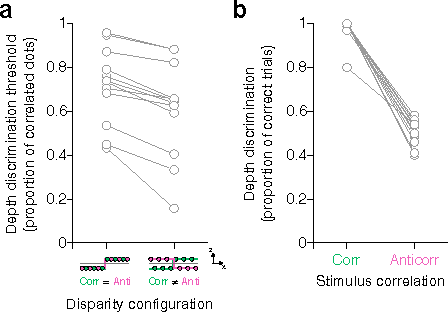
\includegraphics{Fig2}
  \caption[Masking is stronger when correlated and anticorrelated features depict the same disparity.]{Masking is stronger when correlated and anticorrelated features depict the same disparity. Participants (N=12) judged whether the step was closer on the left or right side of the viewed display. I used an adaptive staircase procedure to measure discrimination thresholds for which I varied the proportion of anticorrelated dots in the display. (a) Proportion of correlated dots tolerated by the observers (75\% correct thresholds) for stimuli where correlated and anticorrelated features had the same or the opposite disparity sign. All participants performed better when correlation and anticorrelation carried opposite disparity signs. (b) As a control, I measured performance when observers viewed purely correlated or anticorrelated stereograms. As expected, fully correlated stereograms were trivially discriminated by participants. However, observers performed at chance level for fully anticorrelated stereograms (two-tailed one sample t-test against chance performance, t(11)=0.30, p=0.77). Therefore, anticorrelated features alone did not elicit a reliable depth percept.}
  \label{fig:c2f2}
\end{figure}

It is known that viewing anticorrelated stereograms can potentially elicit rapid vergence eye movements that are contingent on the disparity imposed in such anticorrelated displays \cite{Masson:1997jq}. Because the two conditions differed in the disparity encapsulated in anticorrelated dots (compared to correlated dots), it was important to rule out a potential impact of eye movements in perceptual sensitivity. To do so, I recorded eye movements binocularly while participants performed the main psychophysical experiment. I found no evidence for a differential effect of the anticorrelated disparity signals on binocular eye position (Fig. \ref{fig:c2fs1}). Thus, I conclude that the psychophysical effect reported above is unlikely to be caused by differences in vergence between the two conditions.

\begin{figure}
  \centering
  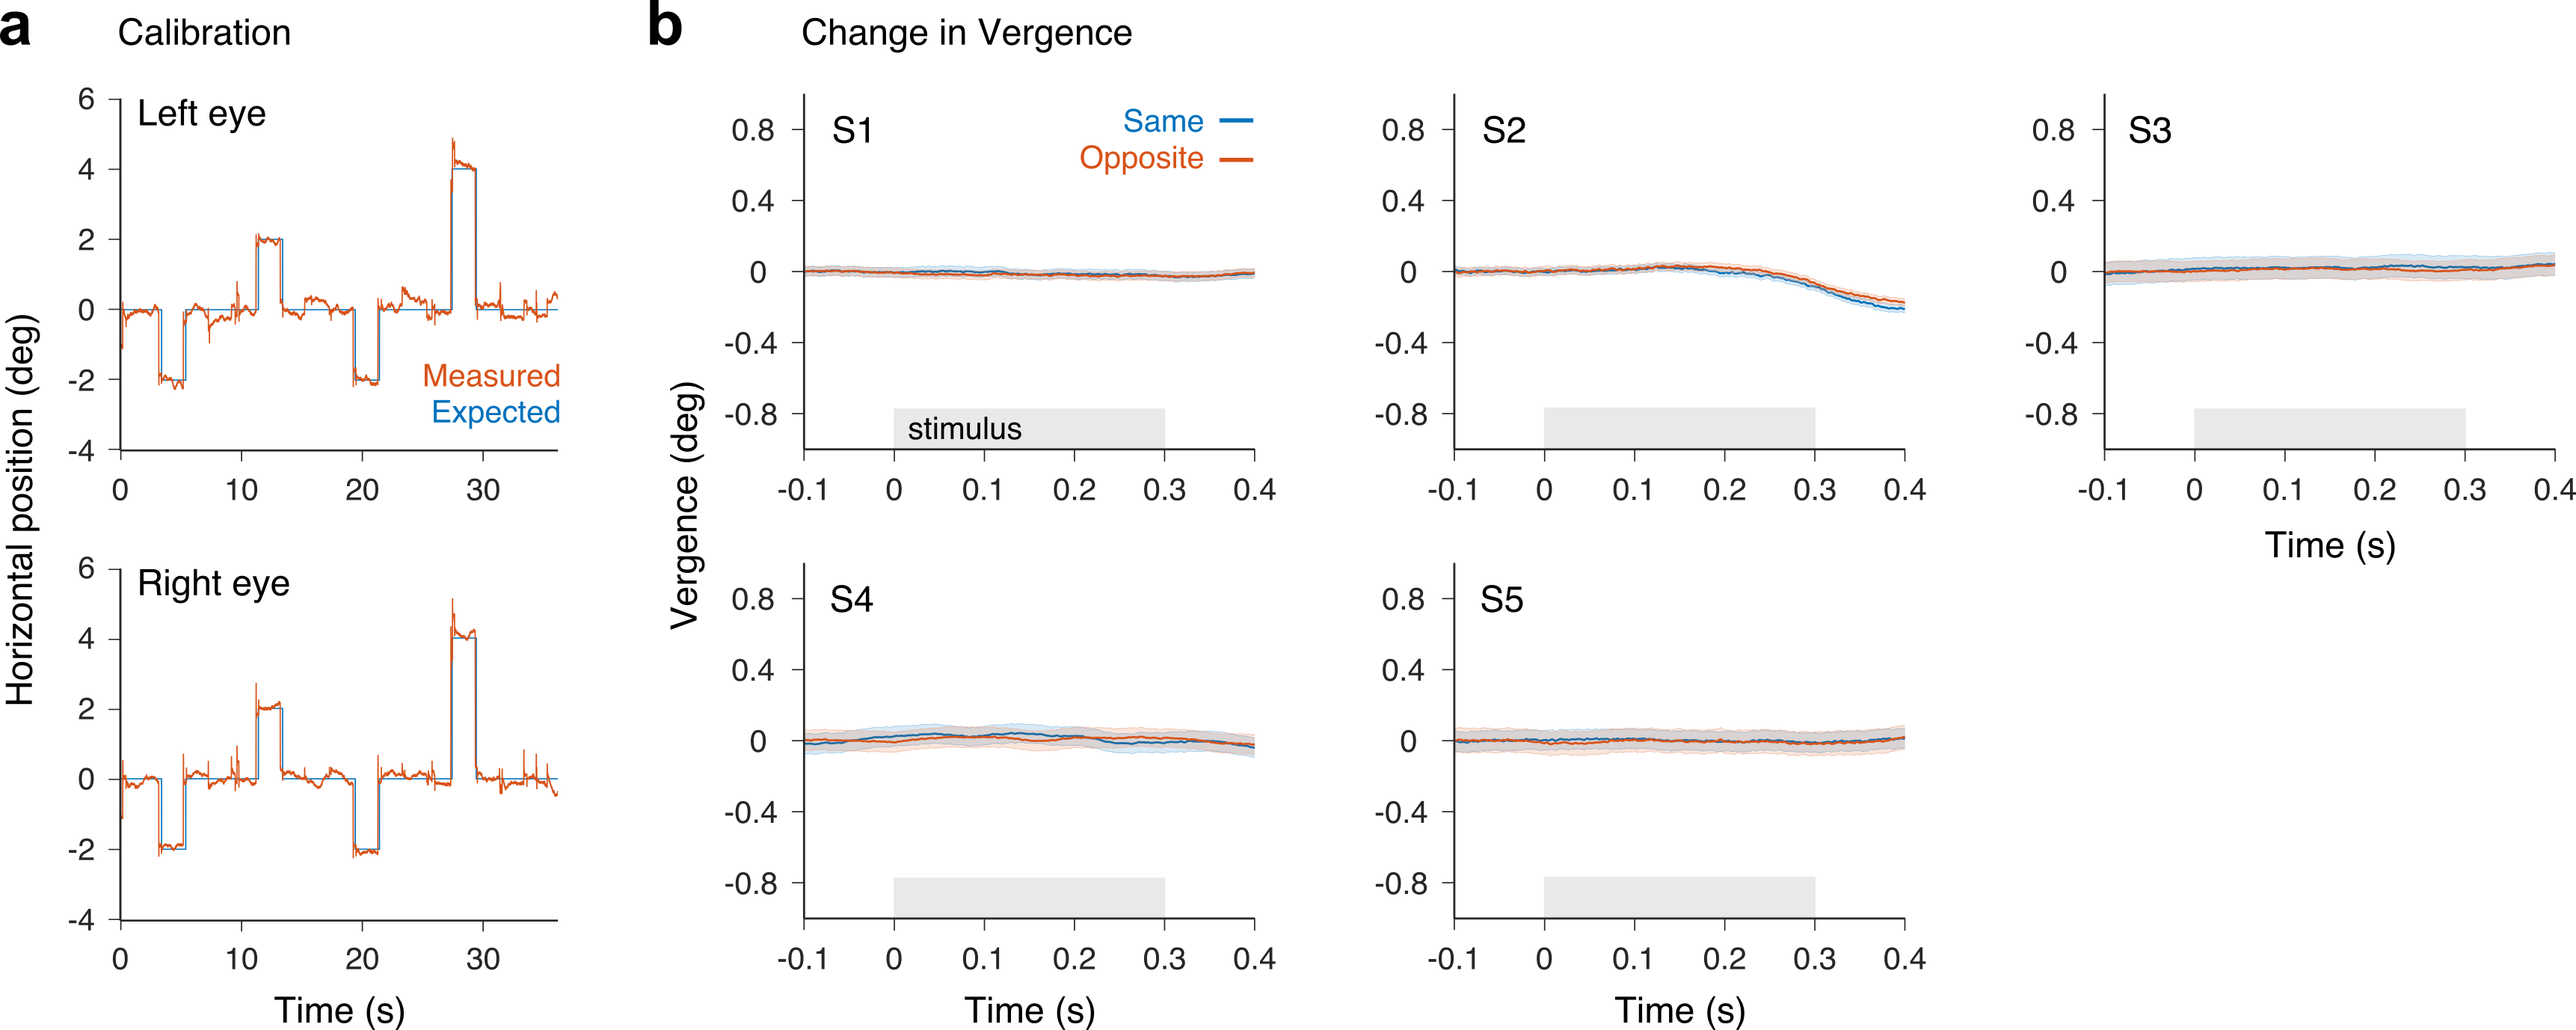
\includegraphics[width=14cm,keepaspectratio]{FigS1}
  \caption[Binocular eye tracking.]{Binocular eye tracking. I recorded binocular eye movements for 5 participants throughout the main experiment to control for potential differences in vergence across conditions. (a) Example eye position trace for the left and right eyes during a calibration block demonstrating eye tracking. (b) Event-related vergence measurements for individual subjects (N=5). Grey time-windows represent stimulus presentation periods. Vergence was not differentially affected by stimulus conditions for any of the subjects (p>0.05; Wilcoxon rank sum test between mean pre-stimulus vergence and vergence at each time point within the stimulus presentation window).}
  \label{fig:c2fs1}
\end{figure}



\subsection{Specificity of the masking effect}
In a series of follow-up experiments, I sought to characterize the specificity of the masking effect in space and time. First, I tested how similar the correlated and anticorrelated disparities should be for masking to be observed. I quantified masking as a function of the difference between the correlated and anticorrelated disparities (Fig. \ref{fig:c2f3}a), and found that masking varies as a function of the disparity separation between the correlated and anticorrelated dots (Fig. \ref{fig:c2f3}b). In particular, masking is maximal when correlated and anticorrelated dots have the same disparity, and there was little masking when they were separated by 6 arcmin of disparity. This suggests that the masking effect is narrowly tuned to the specific disparities conveyed by the anticorrelated portions of the display.

\begin{figure}
  \centering
  \includegraphics{Fig3}
  \caption[Specificity of masking by anticorrelation.]{Specificity of masking by anticorrelation. The masking effect is reduced as the disparity difference between the correlated and anticorrelated elements increases. (a) Observers performed the step-edge depth discrimination task while I parametrically varied the difference between the disparities of correlated and anticorrelated dots. Stimulus illustrations designed to be viewed through red-cyan anaglyphs (red filter over left eye). (b) Proportion of correct choices as a function of the difference between correlated and anticorrelated disparities. Observers are at chance level when correlated and anticorrelated disparities carry the same disparity, but the masking effect gradually decreases --- and eventually disappears for disparity differences greater that 6 minutes of arc. Circles denote proportion of correct choices for disparity differences ranging from 0 to 12 arcmin. Solid lines depict sigmoid curve fits (psignifit 3.0 \cite{Frund:2011aa}).}
  \label{fig:c2f3}
\end{figure}


To probe the specificity of masking further, I relied on the fact that disparity channels in the human visual system are less tightly tuned for larger disparities \cite{TYLER:1975fu,Badcock:1985ly,Lehky:1990fk,Stevenson:1992kx}. In particular, I measured the disparity tuning of masking for different magnitudes of the disparity step-edge (Fig. \ref{fig:c2f4}a), obtaining one psychometric function for each magnitude (Fig. \ref{fig:c2f4}b). I quantified the specificity of masking using the disparity difference at which the observers' performance was half-way between its minimum and maximum value (analogous to the tuning half-width). I found that the tuning width of masking increased (quasi-) linearly with increasing disparity magnitude (Fig. \ref{fig:c2f4}c; Pearson's correlation, R=0.84, N=10, p=0.002; data pooled across subjects). Further, the tuning width values I obtained were remarkably consistent with previous psychophysical data \cite{Stevenson:1992kx} (Fig. \ref{fig:c2f4}c, grey lines) as well as estimates from fMRI recordings \cite{Goncalves:2015aa} (Fig. \ref{fig:c2f4}c, red lines). 


\begin{figure}
  \centering
  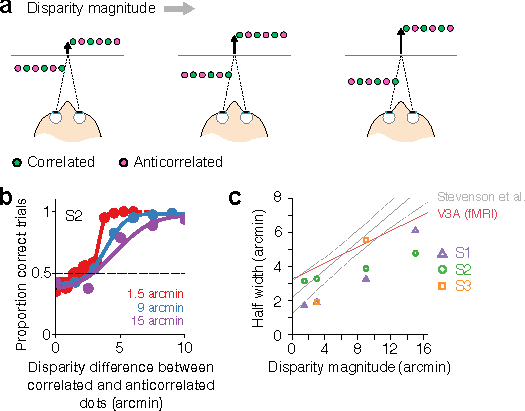
\includegraphics{Fig4}
  \caption[A size-disparity correlation for anticorrelation masking.]{A size-disparity correlation for anticorrelation masking. (a) In addition to varying the distance between correlated and anticorrelated disparities, I also varied the disparity magnitude of the step-edge. (b) Example psychometric curves for different disparity magnitudes for one observer. As a proxy for specificity, I extracted a ``half-width'' parameter by finding the disparity difference at which the psychometric curve was half-way between its minimum and maximum. (c) I found that the effect tuning width, as indexed by the half-width parameter, increases with disparity magnitude. My estimates (coloured symbols) line up well with previous psychophysical estimates of tuning width of disparity channels \cite{Stevenson:1992kx}, as well as with fMRI-metric estimates from area V3A in the human brain \cite{Goncalves:2015aa}. Grey lines represent bootstrapped mean and 95\% CI from reference \cite{Stevenson:1992kx}. Red line represents fMRI-metric estimates from reference \cite{Goncalves:2015aa}.}
  \label{fig:c2f4}
\end{figure}


\subsection{Spatial extent of the masking effect}
We have now seen that (i) the visual system uses disparity information contained in anticorrelated features, and (ii) it does so in a rather selective way. These findings describe the interaction between correlated and anticorrelated features in depth (i.e. along the z-axis; Fig. \ref{fig:c2f3}a-\ref{fig:c2f4}a). Next, I sought to characterize how the masking effect of anticorrelation depends on the visuotopic (i.e. frontoparallel) separation between correlated and anticorrelated features. I assessed this in a simple way by changing the spatial arrangement of correlated and anticorrelated dots in the display (Fig. \ref{fig:c2f5}a). In particular, I measured performance on the step-edge discrimination task when correlated and anticorrelated features were closely intermixed, or more widely separated. I found that the masking effect diminished when the correlated and anticorrelated features were spatially separated from each other (Fig. \ref{fig:c2f5}b), and had virtually disappeared for spatial periods greater than 30 arcmin. These data suggest that the anticorrelation masking effect might be limited by relatively small receptive field sizes, possibly in early visual cortex.


\begin{figure}
  \centering
  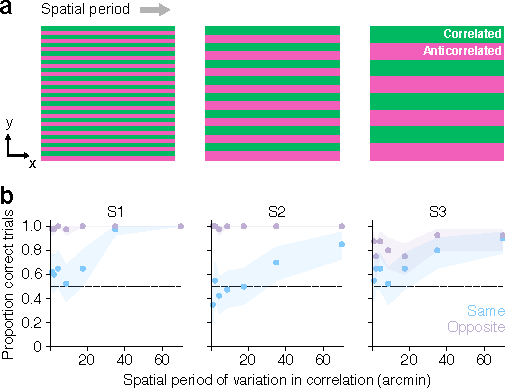
\includegraphics{Fig5}
  \caption[Effect of visuotopic distance between correlated and anticorrelated dots.]{(a) Random-dot stereograms consisted of an even mixture of correlated and anticorrelated dots, but I varied their spatial arrangement along the vertical axis. The arrangement was dictated by a square-wave function with period ranging from 1 to 70 arcmin (seven equally spaced steps in logarithmic scale). This is depicted in cartoon form. (b) Proportion of correct responses as a function of the spatial period of the correlation square-wave for individual subjects. Blue elements depict performance for stimuli where correlated and anticorrelated disparities were equal. Purple elements depict data for stimuli where correlated and anticorrelated dots had disparities of opposite sign. The shaded area indicates bootstrapped 95\% CI. Absence of shaded areas represent no variability in bootstrapped statistic.}
  \label{fig:c2f5}
\end{figure}


\subsection{Asynchrony between correlation and anticorrelation}
Having examined the spatial properties of masking, I now turn to its characterization in time. I recently suggested that neural responses to anticorrelated disparities might be strongly mediated by suppression \cite{Goncalves:2017aa}. To implement this in cortex would entail the use of inhibitory interneurons, imposing an additional synapse (relative to excitation). This entails a temporal delay, and neurophysiological evidence suggests that delayed suppression might be an important mechanism in stereopsis \cite{Tanabe:2011pt,Tanabe:2014ud}. Therefore, I postulated that manipulating the relative time of onset of correlated and anticorrelated dots in the display could modulate the masking effect. In particular, I predicted a stronger masking effect if anticorrelated features precede correlated features, as there is more opportunity to drive suppression before the onset of visual features that drive net excitation.

To test this idea, I manipulated the onset asynchrony between correlated and anticorrelated dots in the RDS, so that anticorrelated dots could lead or lag correlated dots by up to 33 milliseconds (Fig. \ref{fig:c2f6}a). While the relative timing of the correlated and anticorrelated portions of the stimuli was too short for observers to be aware of, I found that observers' performance was consistently worse when anticorrelated dots preceded correlated dots (Fig. \ref{fig:c2f6}b,c). This is compatible with the idea that anticorrelation drives suppression, and that suppression lags excitation.

A potential concern with this experiment is that anticorrelated features might disrupt binocular eye vergence, which, in turn, could alter performance on the depth discrimination task --- particularly given the short stimulus presentation period (133 milliseconds). While this is plausible, the results do not support this view. First, the effect was observed even for very short asynchronies between correlation and anticorrelation. In the shortest asynchrony case, there was only 1 frame (i.e. 8.3 milliseconds) during which I displayed anticorrelated dots alone, which is unlikely to affect vergence. Second, the observers were highly trained to maintain vergence during stereoscopic viewing. Third, stimuli were surrounded by a background pattern to promote a reference for stable vergence throughout the entire experiment. Fourth, I performed an additional experiment for one of the participants where I kept the onset asynchrony constant but increased the total presentation time from 133 to 250 milliseconds, thereby allowing the subject to correct a putative transient disruption of vergence. The effect persisted, suggesting that the masking effect did not depend on the stimulus presentation time.

Finally, I tested whether the effect was specific to anticorrelation, rather than being a generalised metacontrast masking effect \cite{breitmeyer1984visual}. To do so, I included a control condition in which anticorrelated dots in the stimulus were replaced by uncorrelated dots. Like anticorrelated features, uncorrelated dots do not support a coherent depth impression. However, under the proscriptive framework there is a critical difference in that uncorrelated dots do not drive suppression of a particular disparity. As such I did not expect differential masking from adding uncorrelated dots to the display. In line with this logic, I found that the observers' performance did not depend on the onset asynchrony between correlated and uncorrelated dots (Fig. \ref{fig:c2f6}d). This indicates that the temporal masking effect is specific to anticorrelation, which I interpret as a means of driving suppression of particular disparity signals.

\begin{figure}
  \centering
  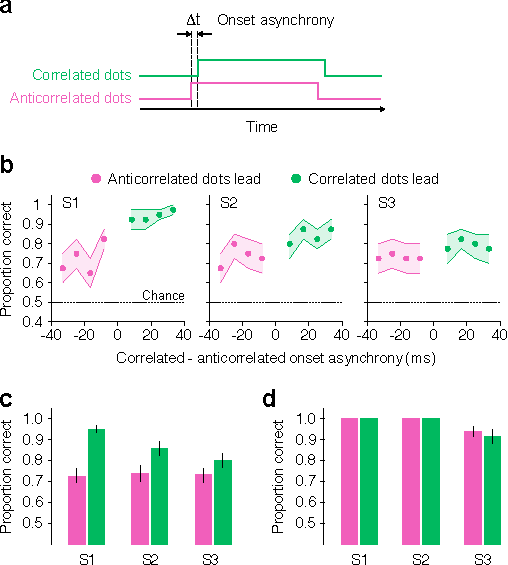
\includegraphics{Fig6}
  \caption[Effect of temporal asynchrony between correlation and anticorrelation.]{Effect of temporal asynchrony between correlation and anticorrelation. (a) I examined the perceptual consequences of varying the relative onset time of correlated and anticorrelated dots. Anticorrelated dots could lead or lag correlated dots by a temporal interval ranging from 8.3 milliseconds (1 monitor refresh frame) to up to 33.3 milliseconds (4 monitor refresh frames). (b) Proportion of correct choices was lower when anticorrelated dots preceded correlated dots (pink elements) compared to when correlated dots led (green elements). Points and shaded regions represent bootstrapped mean and 95\% CI, respectively. (c) Proportion of correct responses for individual subjects obtained by grouping the data in panel b by leading dot type. Performance is worse when anticorrelated dots lead. (d) Proportion of correct responses for a control experiment in which I replaced anticorrelated dots by uncorrelated dots. Bar graphs and error bars represent bootstrapped mean and 95\% CI, respectively.}
  \label{fig:c2f6}
\end{figure}


\section{Discussion}
Our understanding of sensory processing has been guided by the loose intuition that computations and neural representations should resemble perceptual experience. Here I consider a case in which our perceptual experience of a world of solid objects (stereopsis) is enabled by neuronal responses that are selective for features that differ substantially from routine perceptual experience. In particular, I show that visual features that are unlike real objects in the environment, and which have long been understood as nuisance signals that complicate the interpretation of depth, in fact provide information that guides perception.

I tested human participants with stereograms engineered to provide either correlated or anticorrelated signals. My logic was to test the effects of combining information for and against particular depth interpretations. Under the proscriptive framework, anticorrelation provides `what not' information that drives suppression of depth values that are unlikely to have been evoked by the viewed scene. Here I demonstrate the perceptual consequences of doing this: depicting correlated and anticorrelated signals with the same disparity makes the correlated signal harder to see (Fig. \ref{fig:c2f1}e,f; Fig. \ref{fig:c2f2}). This masking effect is tuned to the disparity depicted by the anticorrelated signals, their spatial and temporal configuration. I suggest this reflects the effects of driving suppression of the disparity indicated by the anticorrelated elements. It is important to understand that these stimuli do not isolate correlated vs. anticorrelated signals. Rather, any viewed scene (including correlated RDS) will provide the brain with some visual features that are correlated and others that are anticorrelated. The brain should use the totality of this information (i.e., both dissimilar and similar features) to estimate the most likely interpretation of the scene \cite{Goncalves:2017aa}.

One potential concern with this study is that partially or totally anticorrelated stimuli appear to be quite unnatural. Thus, one may quite rightly question their ecological validity. However, that binocular anticorrelation is a substantial part of the routine diet of the visual system has remained largely ignored. In fact, anticorrelated features occur frequently during natural viewing since multiple visual elements of opposite contrast polarity are often present in the same image. Moreover, anticorrelated disparities often arise when viewing glossy objects relative to non-glossy (but otherwise identical) objects \cite{Muryy:2014hk,Muryy:2016km}. Thus, while the experiment was ran under very controlled conditions, the stimuli used reflect ecologically valid circumstances.

The perception of depth based on stimuli of inverted contrast polarity was first examined by Helmholtz \cite{helmholtz1909physiological}. Several studies have tested the perception evoked by anticorrelation, and suggested that these stimuli generally do support depth perception \cite{BLTJ:BLTJ3954} except in very specific circumstances where a weak percept may emerge \cite{JULESZ:1964ff,Cogan:1993yr,Cumming:1998ib,Read:2000kx,Hibbard2014}. In the rare circumstances where depth perception emerges, the perceived depth sign varies. For instance, very sparse anticorrelated RDS can elicit a veridical disparity percept \cite{Cogan:1993yr,Cumming:1998ib}, whereas very large disparities were reported to elicit a weak and reversed depth percept \cite{Doi:2011ku}. It is known that the firing rates of disparity selective V1 neurons are reliably modulated by disparity in anticorrelated RDS \cite{Cumming:1997ve,Samonds:2013cs}. This has suggested a discrepancy between perception and neurophysiology, with the interpretation being that the responses of V1 neurons to anticorrelated RDS are not closely linked to perception \cite{Cumming:1998ib}.

This study demonstrates that the disparity carried by anticorrelated features is important for perception. I show that the visual system is exquisitely sensitive to differences in the disparity imposed in anticorrelated features (Fig. \ref{fig:c2f3} and \ref{fig:c2f4}). Previous research concluded that correlation computations are negligible for fine disparities, since reversals of depth perception with anticorrelated RDS only occur for coarse disparities \cite{Doi:2011ku}. The results reported here challenge this idea. I show that the visual system is not blind to anticorrelated disparities, even when disparity magnitude of the step-edge was small (1.5 arcmin) (Fig \ref{fig:c2f4}b, c).

Additionally, I show that the effects of anticorrelation are more specific for small disparity magnitudes than they are for large disparity magnitudes (Fig. \ref{fig:c2f4}c). These properties are usually attributed to the detection of similar features in the two eyes \cite{Badcock:1985ly,Lehky:1990fk,Stevenson:1992kx}. Such similarities suggest the existence of common underlying neural machinery responsible for sensing a continuum of binocular correlation: from highly similar to highly dissimilar.
Could the masking effect of anticorrelation be explained by residual perception of depth based on anticorrelated features alone? Control experiments do not suggest this is the case --- observers performed at chance level when I replayed the step-edge stimuli rendered exclusively with anticorrelated dots (Fig. \ref{fig:c2f2}c). Additionally, veridical or reversed depth perception based on anticorrelated features alone would predict differences in performance when the disparity in anticorrelated and correlated dots deviate by the same magnitude, but in opposite directions. By contrast, I found that the perceptual tuning curves (e.g. Fig. \ref{fig:c2f4}b) for opposing directions were strongly correlated (R=0.81, N=100, p<0.001). Together, this suggests that residual perception based on anticorrelated features alone does not explain these results.

It is tempting to speculate about the extent to which models of disparity selectivity in V1 can account for these results. However, the link is not straightforward. The energy model can account for both veridical and reversed depth ``percepts'' for anticorrelated stereograms, depending on the particular parametrization of the energy model \cite{Read:2002kx,Henriksen_2016}. This is also the case for the binocular likelihood model \cite{Goncalves:2017aa}. As others have concluded\cite{Cumming:1998ib,Janssen:2003fk}, additional processing of stereoscopic information that supports perception likely takes place in extrastriate visual cortex.

It is important to note that I found considerable between-subject differences in the extent to which individuals could tolerate anticorrelated elements added to the display (Fig. \ref{fig:c2f2}a; i.e., note the absolute position of each participant's data on the ordinate axis, rather than the relative difference between the two conditions). While I found that the contrast between Figures \ref{fig:c2f1}e and \ref{fig:c2f1}f works well for ~90\% of the two hundred or more people I have tried this demonstration on, quantifying this effect in a laboratory setting clearly challenges participants' visual systems. Experienced psychophysical observers could tolerate enough anticorrelation added to the stimuli to give sufficient experimental dynamic range to explore the effects in detail. It is known that training can have profound effects on stereoscopic vision \cite{Chowdhury:2008aa,Chang:2014ns}. It is possible that the suppression produced from anticorrelation is so strong in naive participants that it becomes difficult to tolerate even a small amount, especially under the brief presentation durations needed for well-controlled psychophysical testing.

The neural computations that support stereoscopic vision likely involve suppression \cite{Goncalves:2017aa,Samonds:2013cs,Haefner:2008jg,Burge:2014qj,Jaini158741}, especially for anticorrelated disparities \cite{Goncalves:2017aa}. Neurophysiological data suggest that suppressive input onto disparity detectors is delayed with respect to excitation \cite{Tanabe:2014ud}. Thus, I hypothesize that the response to anticorrelated stimuli may be partly mediated by delayed suppression. In agreement with this, I show that `front-loading' the visual system with anticorrelated dots, putatively eliminating the delay between excitation and suppression, has a greater effect on performance than when anticorrelated dots are presented after correlated dots (Fig. \ref{fig:c2f6}b,c). More generally, these data suggest that suppression shapes the tuning of disparity detectors --- an idea that has received strong neurophysiological support \cite{Tanabe:2011pt,Tanabe:2014ud,Nieder:2001jl}.

Humans can detect variations in disparity over spatial regions as small as 4-8 arcmin \cite{Harris:1997kx,Banks:2004oh}, a resolution measure that has been linked to the size of V1 receptive fields \cite{Nienborg:2004ra}. Although consistent with the size of V1 receptive fields, these results suggest that disparity in anticorrelated features might be pooled over a somewhat greater extent. I observed strong masking from anticorrelation for signals separated by up to 20 arcmin (Fig. \ref{fig:c2f5}b). As a result, it is possible that the interaction between disparity in correlated and anticorrelated features spans a greater extent than the interaction between disparity in correlated features. This would point towards a form of extra-classical contextual modulation effect, perhaps implemented by means of a centre-surround-like receptive field organization for correlated and anticorrelated disparities. However, further psychophysical testing is needed to directly answer this question. To my knowledge, neurophysiological investigations have not yet addressed this, but recent work suggests that complex cells rely on extensive pooling \cite{Sasaki:2010pi,Kato:2016fk}.

\section{Conclusion}

Neural responses to anticorrelated visual features have long appeared surprising: a physical feature in the environment will not project anticorrelated intensities to the two eyes, and viewing anticorrelated displays does not support a robust perceptual interpretation. As such, these signals were thought to complicate the perceptual interpretation of depth. By contrast, here I show that they guide perception: using ``what not'' information to suppress unlikely interpretations of the viewed scene, confirming the predictions put forward at the end of Chapter 2. 

So far, I have focused on (i) the role of V1 in disparity processing and (ii) the corresponding implications for perception. However, while area V1 is likely to play a critical role in processing binocular disparities, evidence from neurophysiological and neuroimaging studies suggests that neural activity in V1, alone, cannot account for perceptual observations \cite{Cumming:1999zr,Preston:2008dg,Nienborg:2014fu}. Thus, over the past decades, there has been a great deal of interest in understanding which extrastriate visual areas support stereopsis. In particular, functional magnetic resonance imaging studies have consistently found that stereopsis recruits dorsomedial areas in the human brain (especially V3A) \cite{Backus:2001ly,Tsao:2003lk,Preston:2008dg}. In the next chapter, I set out to test if dorsomedial visual cortex contains specialized cortical architecture for stereopsis. In particular, I leverage the power of ultra-high field magnetic resonance imaging to test for the presence of persistent and systematic cortical organization, and then assess how well these measurements account for the capabilities and limitations of stereoscopic perception.


% ------------------------------------------------------------------------

%%% Local Variables: 
%%% mode: latex
%%% TeX-master: "../thesis"
%%% End: 
